\documentclass{article}

\usepackage{tikz}
\usetikzlibrary{arrows,arrows.meta,calc,fit}
\usetikzlibrary{positioning,patterns,matrix}
\usetikzlibrary{decorations.markings,decorations.pathreplacing,decorations.pathmorphing}
\usetikzlibrary{shapes,shapes.arrows,shapes.geometric,shapes.multipart}

\tikzstyle{ndint} = [draw, line width=1pt, color=teal, shape=rectangle, minimum size=20pt,inner sep=0pt, text=black]
\tikzstyle{ndout} = [draw, line width=1pt, shape=circle, color=blue, minimum size=20pt,inner sep=0pt, text=black]
\tikzstyle{ndlat} = [draw, line width=1pt, shape=circle, color=red, minimum size=20pt,inner sep=0pt, text=black]
\tikzstyle{arint} = [style={->,>=Latex,thick,teal}]
\tikzstyle{arout} = [style={->,>=Latex,thick,blue}]
\tikzstyle{arlout} = [style={->,>=Latex,thick,red}]
\tikzstyle{arlat} = [style={<->,>=Latex,thick,red}]

\begin{document}
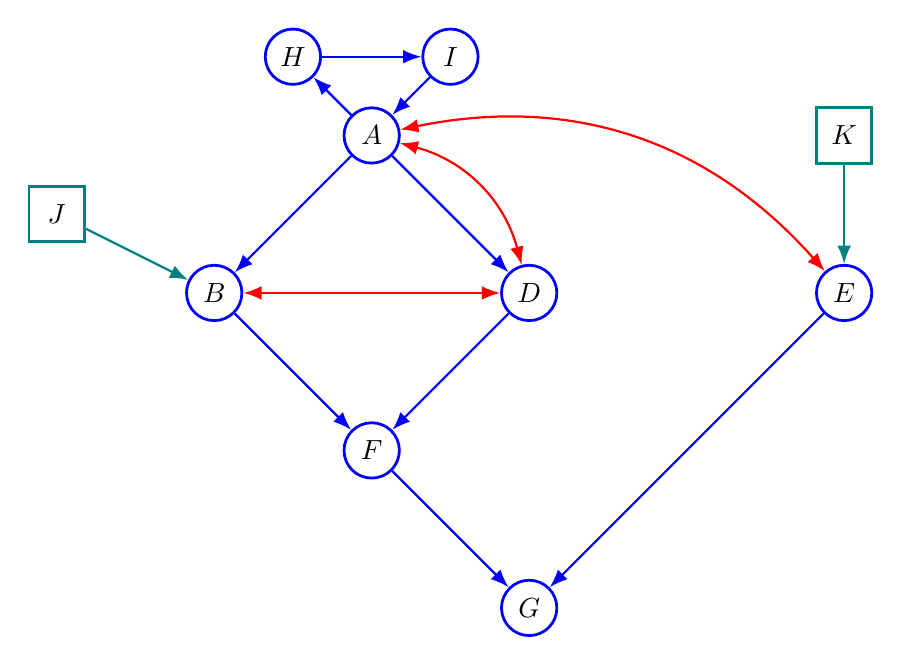
\begin{tikzpicture}[scale=1, transform shape]
	\node[ndout] (v1) at (5,5) {$A$};
	\node[ndout] (v2) at (3,3) {$B$};
	\node[ndout] (v3) at (7,3) {$D$};
	\node[ndout] (v7) at (11,3) {$E$};
	\node[ndout] (v5) at (5,1) {$F$};
	\node[ndout] (v6) at (7,-1) {$G$};
	\node[ndout] (v12) at (4,6) {$H$};
	\node[ndout] (v13) at (6,6) {$I$};
	\node[ndint] (v4) at (1,4) {$J$};
	\node[ndint] (v11) at (11,5) {$K$};
	\draw[arint] (v4) to (v2);
	\draw[arint] (v11) to (v7);
	\draw[arlat, bend left] (v1) to (v3);
	\draw[arlat, bend left] (v1) to (v7);
	\draw[arlat] (v2) to (v3);
	\draw[arout] (v1) to (v2);
	\draw[arout] (v1) to (v12);
	\draw[arout] (v12) to (v13);
	\draw[arout] (v13) to (v1);
	\draw[arout] (v1) to (v3);
	\draw[arout] (v2) to (v5);
	\draw[arout] (v3) to (v5);
	\draw[arout] (v5) to (v6);
	\draw[arout] (v7) to (v6);
\end{tikzpicture}
\end{document}